% !TEX root = main.tex
\begin{figure}[htbp]
\centering
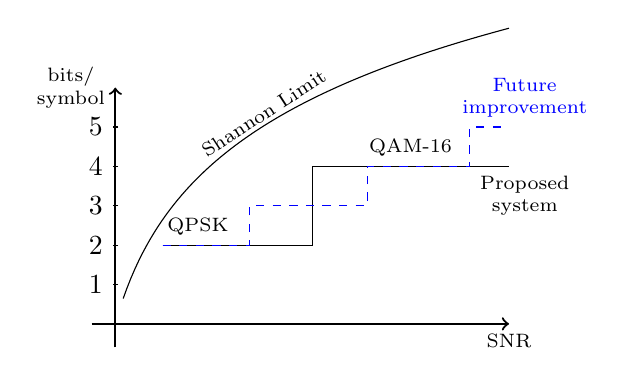
\begin{tikzpicture}
% Coordinate system
\coordinate (origo) at (0,0);

\draw[->, thick] (-0.3, 0) -- (5, 0) node[below, font=\scriptsize]{SNR};
\draw[->, thick] (0, -0.3) -- (0, 3) node[left, align=center, font=\scriptsize]{bits/\\symbol};

\foreach \x in {1, 2, 3, 4, 5}
   \draw (1pt, 0.5*\x cm) -- (-1pt, 0.5*\x cm) node[anchor=east] {$\x$};
   
% \draw (2.5, 1pt) -- (2.5, -1pt) node[anchor=north] {$\left[\frac{E_b}{N_0}\right]$};

%Lines
\draw[] (0.6, 1) -- node[above, font=\scriptsize, xshift=-0.5cm]{QPSK} (2.5,1) -- (2.5, 2) -- node[above, font=\scriptsize]{QAM-16} (5, 2) node[below, xshift=0.2cm, align=center, font=\scriptsize](c2){Proposed \\ system}; 
\draw[dashed, blue] (0.6, 1) -- (1.7, 1) -- (1.7, 1.5) -- (3.2, 1.5) -- (3.2, 2) -- (4.5, 2) -- (4.5, 2.5) -- (5, 2.5) node[above, xshift=0.2cm, align=center, font=\scriptsize](c2){Future \\ improvement}; 

\draw plot [domain=0.1:5,samples=100] (\x,{log2(1 + 2.5*\x)});
\draw (2, 2.5) node[above, font=\scriptsize, rotate=33]{Shannon Limit};


\end{tikzpicture}
\caption{Qualitative illustration of the adaptive quality concept}
\label{fig:concept}
\end{figure}